%%% Thesis Introduction --------------------------------------------------
\chapter{Game Theory, Cooperation and Fitness}
\ifpdf
    \graphicspath{{GameTheory/Figs/PNG/}{GameTheory/Figs/PDF/}{GameTheory/Figs/}}
\else
    \graphicspath{{GameTheory/Figs/EPS/}{GameTheory/Figs/}}
\fi
 Evolution is usually described as a fierce competition between individuals, that leads to a selfish behavior as, for example  the competition among lions for females, but it has been seen that in many biological systems evolution leads also to cooperative behaviors between individuals\cite{Dunny2008}, for example when bacteria gather in a biofilm to help each other, or in cooperation among humans in a work team. 

Natural selection can leads to cooperation if it  implies a higher benefit than that when individuals are selfish. A population of only cooperators can then be invaded by a cheater if behaving like that has more benefit, or the opposite situation where cheaters are invaded by cooperators. The mechanisms that leads to one of those behaviors in a population of individuals depend on the biological system.   

Some scientist have proposed models to described the selection of cooperation and behavior interactions among organisms. This science field has been called evolutionary game theory. For example  Martin A. Nowak,  who has worked in evolutionary dynamics,  has proposed five mechanisms for the evolution of cooperation based on  game theory, where the benefit of cooperating or defecting is related to the fitness of individuals\cite{Nowak2011,Shoresh2011}. The mechanisms are: kin selection, direct reciprocity, indirect reciprocity, network reciprocity and group selection. The last one , group selection, describes the evolution of cooperation in individuals of different groups that are on competition.

%The group selection model is based in a fixed grade of cooperation, which means that it is deterministic, but in a biological system each individual is going to cooperate in different degrees due to the phenotype variability, although in isogenic groups. This is an effect of the gene expression noise. For example the noise expression noise affects the fitness of organisms when its fitness depends of some phenotype advantage that is generate by a gene or group of genes, the increase in the gene noise expression can leads to a decrement of the total fitness.  Including phenotypic variability to Nowak's model allows an approach more realistic to the evolution of cooperation, and detailed simulations of competition populations of cooperators and defectors would allow to characterize the importance of phenotypic variability and its utility as an evolutive strategy.  


Differences between evolutionary game theory and classical game theory are essential. Classical theory considers rational players thinking about others strategies, which becomes an infinite iterating game \cite{Traulsen2009}. In evolutionary game theory organisms are considered not rational, and strategies spreads depending on the utility that they give to the players; they can be imitated or inherited.   

%%% ----------------------------------------------------------------------
\section{Fitness Due to Cooperate-Defect}
When organisms have interaction in some environment where each of them have the possibility of different strategies or behaviors, from those interactions each individual in the biological system will get an utility. In the simplest situation imagine  two different organisms that have the option of two behaviors: cooperate and defect. For example in sea there are two fish, the white shark and Pilot fish, that cooperate each other.  The White shark can let Pilot fish to eat the parasites on its skin. Therefore it is said that if the shark lets it eat from its skin, it cooperates, and the Pilot fish cooperates when it cleans shark's skin. 
\begin{figure}[H]
 \begin{center}
    \leavevmode
    \ifpdf
      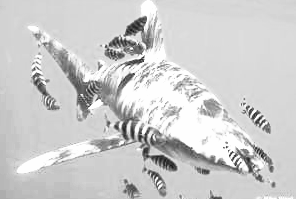
\includegraphics[width=10cm,height=7cm]{mutualism.png}
    \else
     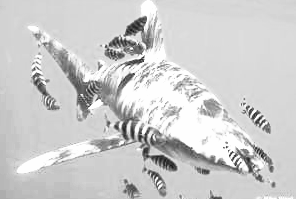
\includegraphics[width=10cm, height=7cm]{mutualism.png}
    \fi
    \caption{\footnotesize Illustration of cooperation between White shark and Pilot fish(www.pioneermindset.wordpress.com).}  
    \label{Fig51}
  \end{center}
  \end{figure}

The utilities of this interaction can be visualize in a payoff matrix.

\begin{equation*}
\begin{matrix}
    & Pilot\; fish \\
 White\; shark & {\bordermatrix{~ & C& D \cr
                            C & A_{shark} & B_{shark} \cr
                            D & C_{shark} & D_{shark} \cr}} 
 \end{matrix}\;\;\;
 \begin{matrix}
    & White \; shark \\
 Pilot\; fish & {\bordermatrix{~ & C& D \cr
                            C & A_{fish} & B_{fish} \cr
                            D & C_{fish} & D_{fish} \cr}} 
\end{matrix}
\end{equation*}

Where the elements of the left hand matrix are the utilities for the shark,  and the right hand matrix has the utilities for the Pilot fish. This utility of the interaction represents a contribution to the fitness of each individual. For the White shark, it will get a skin clean of parasites, increasing its life time and possibility of reproduction. For the Pilot fish, it will get a source of food and protection from bigger predators. Both organisms can get a larger per capita reproduction rate from the altruistic act.

As we see in the last matrices, a matrix  is needed  for the utilities of each individual, but in the case where the utilities from the interaction are symmetric just one payoff matrix  is used:
\begin{equation}\label{5.1}
\bordermatrix{~ & C & D \cr
             C & R & S \cr
              D & T & P \cr}. 
\end{equation}
An example of this symmetric situation, is  a group of bacteria that have pair interactions, where each time that two bacteria meet they have the options of cooperate producing an enzyme for processing food, or defect taking food without  spend energy producing the enzyme. This interaction has a benefit $b$ and a cost $c$ for producing the enzyme. Thus, the  payoff matrix of this game is
\begin{equation*}
\bordermatrix{~ & C & D \cr
             C & b-c & -c \cr
              D & b & 0\cr}, 
\end{equation*}
where it can be observed that the strategy with the largest utility is defecting, but if this strategy invades the group, no bacterium will have a benefit.

Now let us examine how the process of selection works in game theory. Imagine a group of size $n$ with $i$ individuals that cooperate and $n-i$ that defect. The expected payoff $\pi_{C}$ of cooperators due to pairwise encounters with the rest of individuals in the group is
\begin{equation}
 \pi_{C}=\frac{R(i-1)+S(n-i)}{n-1}.
\end{equation}
This average utility will represents a reproductive rate for the individuals with the strategy of cooperation. Usually fitness is  a linear function like
\begin{equation}
f_{C}=1-w+w\pi_{C},
\end{equation}
where $w$ is called the intensity of selection, and represents how much the game contributes to selection process. For example, for $w=0$ the competition reduces to neutral drift and the game has not effect on the fitness.



There is another function of fitness that is usually used, this is an exponential function of expected payoff $\pi_{C}$,
\begin{equation}
f_{C}=e^{w\pi_{C}}.
\end{equation}
This function is usually used for analytical results of fixation probabilities when intensity of selection is large.

Then in summary, in a group of size $n$ and $i$ cooperators, the expected payoff and fitness for a defector will be:
\begin{equation}
\pi_{D}=\frac{Ti + P(n-i-1)}{n-1}\;\:\:\; f_{D}=1-w+w\pi_{D}.
\end{equation} 
 
Systems where there is not fitness due to interaction and it is intrinsic to each type of organism, as random drift also can be written in a payoff matrix, and doing the algebraic calculations get same transitions probabilities. Then for neutral drift
\begin{equation*}
\bordermatrix{~ & A & B \cr
             A & 1 & 1 \cr
              B & 1 & 1 \cr} 
\end{equation*}
 and for random drift
 \begin{equation*}
\bordermatrix{~ & A & B \cr
             A & r & r \cr
              B & s & s \cr}. 
\end{equation*}
Let us calculate $\pi_A$ in the case that $w=1$ for random drift.
\begin{equation*}
f_{A}=\pi_A=\frac{r(i-1)+r(n-i)}{n-1}=r\;\; and \;\; f_{B}=s
\end{equation*}
We have seen above examples of cooperation among different species, but the interest of this work is to study how cooperation evolves among individuals of the same specie, as humans or yeast. 

 
\section{Fixation Probability}
For fixation probability the same procedure is used  as for random drift, with the difference that $f_{C,D}$ is a function of the frequency $i$. First of all, we should define $P_{i,i+1}$ and $P_{i,i-1}$:
\begin{equation}
P_{i,i+1}=\frac{f_{C}i}{f_{C}i+f_{D}(n-i)}\frac{n-i}{n}.
\end{equation} 


Again the equation for $\rho_{i}$ is 
\begin{equation}\label{5.9}
\rho_{i}=\rho_{i}P_{i,i} + \rho_{i-1}P_{i,i-1} + \rho_{i+1}P_{i,i+1}
\end{equation}   
replacing the new variable $x_{i}=\rho_{i}-\rho_{i-1}$.
\begin{equation}
P_{i,i-1}x_{i}=P_{i,i+1}x_{i+1}
\end{equation}
with the conditions
\begin{equation}
 x_0 = 0\;\;\;\; and\;\;\;\; \sum_{i=1}^{n}x_i =1,
 \end{equation}
 
\begin{equation}
x_{i+1}=x_{i}\frac{P_{i,i-1}}{P_{i,i+1}}, \;\;\;\; 0<i
\end{equation}
by induction $x_{i}$ in terns of $\rho_{1}$ is:
\begin{equation}
x_{i}=\rho_{1}\prod\limits_{j=1}^{i-1}\frac{P_{j,j-1}}{P_{j,j+1}}.
\end{equation}
Then replacing (5.13) in (5.11) $\rho_1$ is
\begin{equation}\label{5.14}
\rho_1 =\frac{1}{1+\sum\limits_{i=2}^{n}\prod\limits_{j=1}^{i-1}\frac{P_{j,j-1}}{P_{j,j+1}}},
\end{equation} 
and finally since $\rho_i= \sum\limits_{j=1}^{i}x_j$;
\begin{equation}
\rho_i = \rho_1(1+\sum\limits_{j=2}^{i}\prod\limits_{m=1}^{j-1}\frac{P_{m,m-1}}{P_{m,m+1}}).
\end{equation} 
Now with $\rho_1$ it is possible calculate $\rho_i$. Since $\rho_i=\sum\limits_{j=1}^{i}$
\begin{equation}
\rho_i =\sum\limits_{j=1}^{i}\rho_{1}\prod\limits_{m=1}^{j-1}\frac{P_{m.m-1}}{P_{m,m+1}}=\rho_{1}\left( 1+ \sum\limits_{j=1}^{i-1}\prod\limits_{m=1}^{j}\frac{P_{m,m-1}}{P_{m,m+1}}\right)
\end{equation}
Therefore
\begin{equation}
\rho_i = \frac{1+\sum\limits_{j=2}^{i}\prod\limits_{m=1}^{j-1}\frac{P_{m,m-1}}{P_{m,m+1}}}{1+\sum\limits_{i=2}^{n}\prod\limits_{j=1}^{i-1}\frac{P_{j,j-1}}{P_{j,j+1}}}.
\end{equation}
For weak selection $w\ll 1$ the  expression Eq. \eqref{5.14} for $\rho_1$ can be reduced to a simpler form. Starting with the ratio of the transition probabilities, that is
\begin{equation}
\frac{P_{i,i-1}}{P_{i,i+1}}=\frac{f_D}{f_C}=\frac{1-w+w\pi_D}{1-w+w\pi_C}.
\end{equation} 
Now the term that need to be simplified in $\rho_1$ is the summation
\begin{equation}
\sum\limits_{k=1}^{n-1}\prod\limits_{j=1}^{k}\frac{f_D(j)}{f_C(j)},
\end{equation}
where just the linear terns in the product will be considered. For $k=2$ the product is 
\begin{equation}
\prod\limits_{j=1}^{2}\frac{f_D(j)}{f_C(j)}=\frac{(1-w+w\pi_D(1))(1-w+w\pi_D(2))}{(1-w+w\pi_C(1))(1-w+w\pi_C(2))}\approx \frac{1-2w+w(\pi_D(1)+\pi_D(2))}{1-2w+w(\pi_C(1)+\pi_C(2))},
\end{equation}
and for $k=3$
\begin{equation}
\prod\limits_{j=1}^{3}\frac{f_D(j)}{f_C(j)}\approx \frac{1-3w+w(\pi_D(1)+\pi_D(2)+\pi_D(3))}{1-3w+w(\pi_C(1)+\pi_C(2)+\pi_C(3))}.
\end{equation}
Then by induction:
\begin{equation}
\prod\limits_{j=1}^{k}\frac{f_D(j)}{f_C(j)}\approx \frac{1-kw+w\sum\limits_{j=1}^{k}\pi_D(j)}{1-kw+w\sum\limits_{j=1}^{k}\pi_C(j)}.
\end{equation}
The summations over $\pi_C$ and $\pi_D$
\begin{equation}\label{5.23}
\sum\limits_{j=1}^{k}\pi_D(j)=\frac{1}{n-1}(k(Pn-P)+(T-P)\sum\limits_{j=1}^{k}j)\;\; , \;\sum\limits_{j=1}^{k}\pi_C(j)=\frac{1}{n-1}(k(Sn-R)+(R-S)\sum\limits_{j=1}^{k}j)
\end{equation}
Using  Gauss summation formula
\begin{equation}\label{}
\sum\limits_{j=1}^{k}j=\frac{k(k+1)}{2}
\end{equation}
in Eq. \eqref{5.23}, we get that the summation in the denominator of $\rho_1$ is
\begin{equation}\label{5.25}
\sum\limits_{k=1}^{n-1}\frac{1-w+\frac{wk}{n-1}(Pn-P+\frac{(T-P)}{2}(k+1))}{1-w+\frac{wk}{n-1}(Sn-R+(R-S)\frac{(k+1)}{2})}
\end{equation}
Now the last simplification is done by using the binomial approximation
\begin{equation}
(1+x)^{\alpha}\approx 1+\alpha x\;,\; x\ll1.
\end{equation} 
Then Eq. \eqref{5.25} becomes
\begin{equation}
\sum\limits_{k=1}^{n-1}\left(1+\frac{wk}{n-1}(Pn-P+ \frac{T-P}{2}(k+1)+Sn-R+(R-S)\frac{(k+1)}{2}) \right),
\end{equation}
and using the summation formula
\begin{equation}
\sum\limits_{k=1}^{n}k^2 =\frac{n(n+1)(2n+1)}{6},
\end{equation} 
it is equal to
\begin{equation}
n-1+\frac{wn}{2}\left( (Pn-P+Sn-R)+(R-S+T-P)\left(\frac{1}{2}+\frac{(2n-1)}{6}\right)\right).
\end{equation}
Therefore $\rho_1$ is written as
\begin{equation}
\rho_1 =\frac{1}{n\left(1+ \frac{w}{2}\left( (Pn-P+Sn-R)+(R-s+T-P)(\frac{1}{2}+\frac{(2n-1)}{6})\right)\right)},
\end{equation}
and using again the binomial approximation
\begin{equation}\label{5.29}
\rho_1=\frac{1}{n}-\frac{w}{n2}\left[ (Pn-P+Sn-R)+(R-s+T-P)(\frac{1}{2}+\frac{(2n-1)}{6})\right].
\end{equation}
The fixation probability $\rho_D$ for a defector in a population of $n-1$ cooperators is
\begin{equation}
\rho_D=1-\rho_{n-1},
\end{equation}
and the approximation for weak selection is
\begin{equation}\label{5.31}
\rho_D=\frac{1}{n}+\frac{w}{6n}\left[ 4R-S-T-2P+n(-2R-S+2T+P)\right].
\end{equation}
\section{Fixation Times}
Taking the equations Eq. \eqref{4.36} and \eqref{4.39}
\section{Group Selection}
\cite{Goodnight1997a} \cite{Bower2004}\cite{Dunny2008}\cite{Wade1976}\cite{Shoresh2011}\cite{Nowak2011}\cite{Traulsen2006a}\cite{Gore2009}

In biological systems natural selection does not happen only at the level of individuals; it also happens at the level of groups of individuals\cite{Wade1976}, where the groups with larger average fitness will proliferate splitting in new groups of individuals with the same behavior or physical advantage. This phenomena of group selection is also observed in social systems. For example, competitions between working teams, or the alliance  among enterprises to get any common benefit  that they can not get working individually. At the biological level, group selection has an interesting example and commercial use as described by (Graig and Muir $1996$)\cite{Goodnight1997a} , they made observations on the selection  on chickens  groups in a farm, where chickens groups that do not fight among themselves are selected to have new offsprings, which will be introduced in the farm because they will behave as their parents, and do not faight others inside the cages. The utility of this strategy, is an increasing in egg production.
    
 Group selection is a mechanism for the emergence of cooperative behaviors\cite{Nowak2011}. Some examples of this fact are  given  in \cite{Dunny2008,Bower2004, Gore2009}, where bacteria gather to produce enzymes  needed to process  some food source in the environment. Cheating could be a better strategy individually , but the group needed by a population fraction contributing to the group goods, makes that cooperating producing enzymes fixed in population.  
     
     This process of selection at a second level is simulated using a modified Moran process, that is as follows\cite{Traulsen2006a,Shoresh2011}. In a population of $m$ groups of maximum size $n$, where individuals have interaction only with others in their group. At each time step one individual of the entire population is selected for reproduction, and the new offspring will added to the group of such individual. When this group reaches the maximum amount of population $n$, with probability $q$ it splits randomly in two groups, and a random group is chosen to be replaced by the new offspring group. Finally with a probability $1-q$, this group does not split, and one individual from it is chosen randomly to be replaced by the new offspring (Figure \ref{Fig5.2}). 
 
 
 Even though group selection is usually considered as a mechanisms for the emergence of cooperation and social behaviors, it is also involved in the evolution of phenotypic traits\cite{Wade1976,Traulsen2005}, which can be influenced by group selection. As an example of this, a simulation of random drift with group selection will be shown later.
 
  \begin{figure}[H]
\begin{center}$
\begin{array}{cc}
a)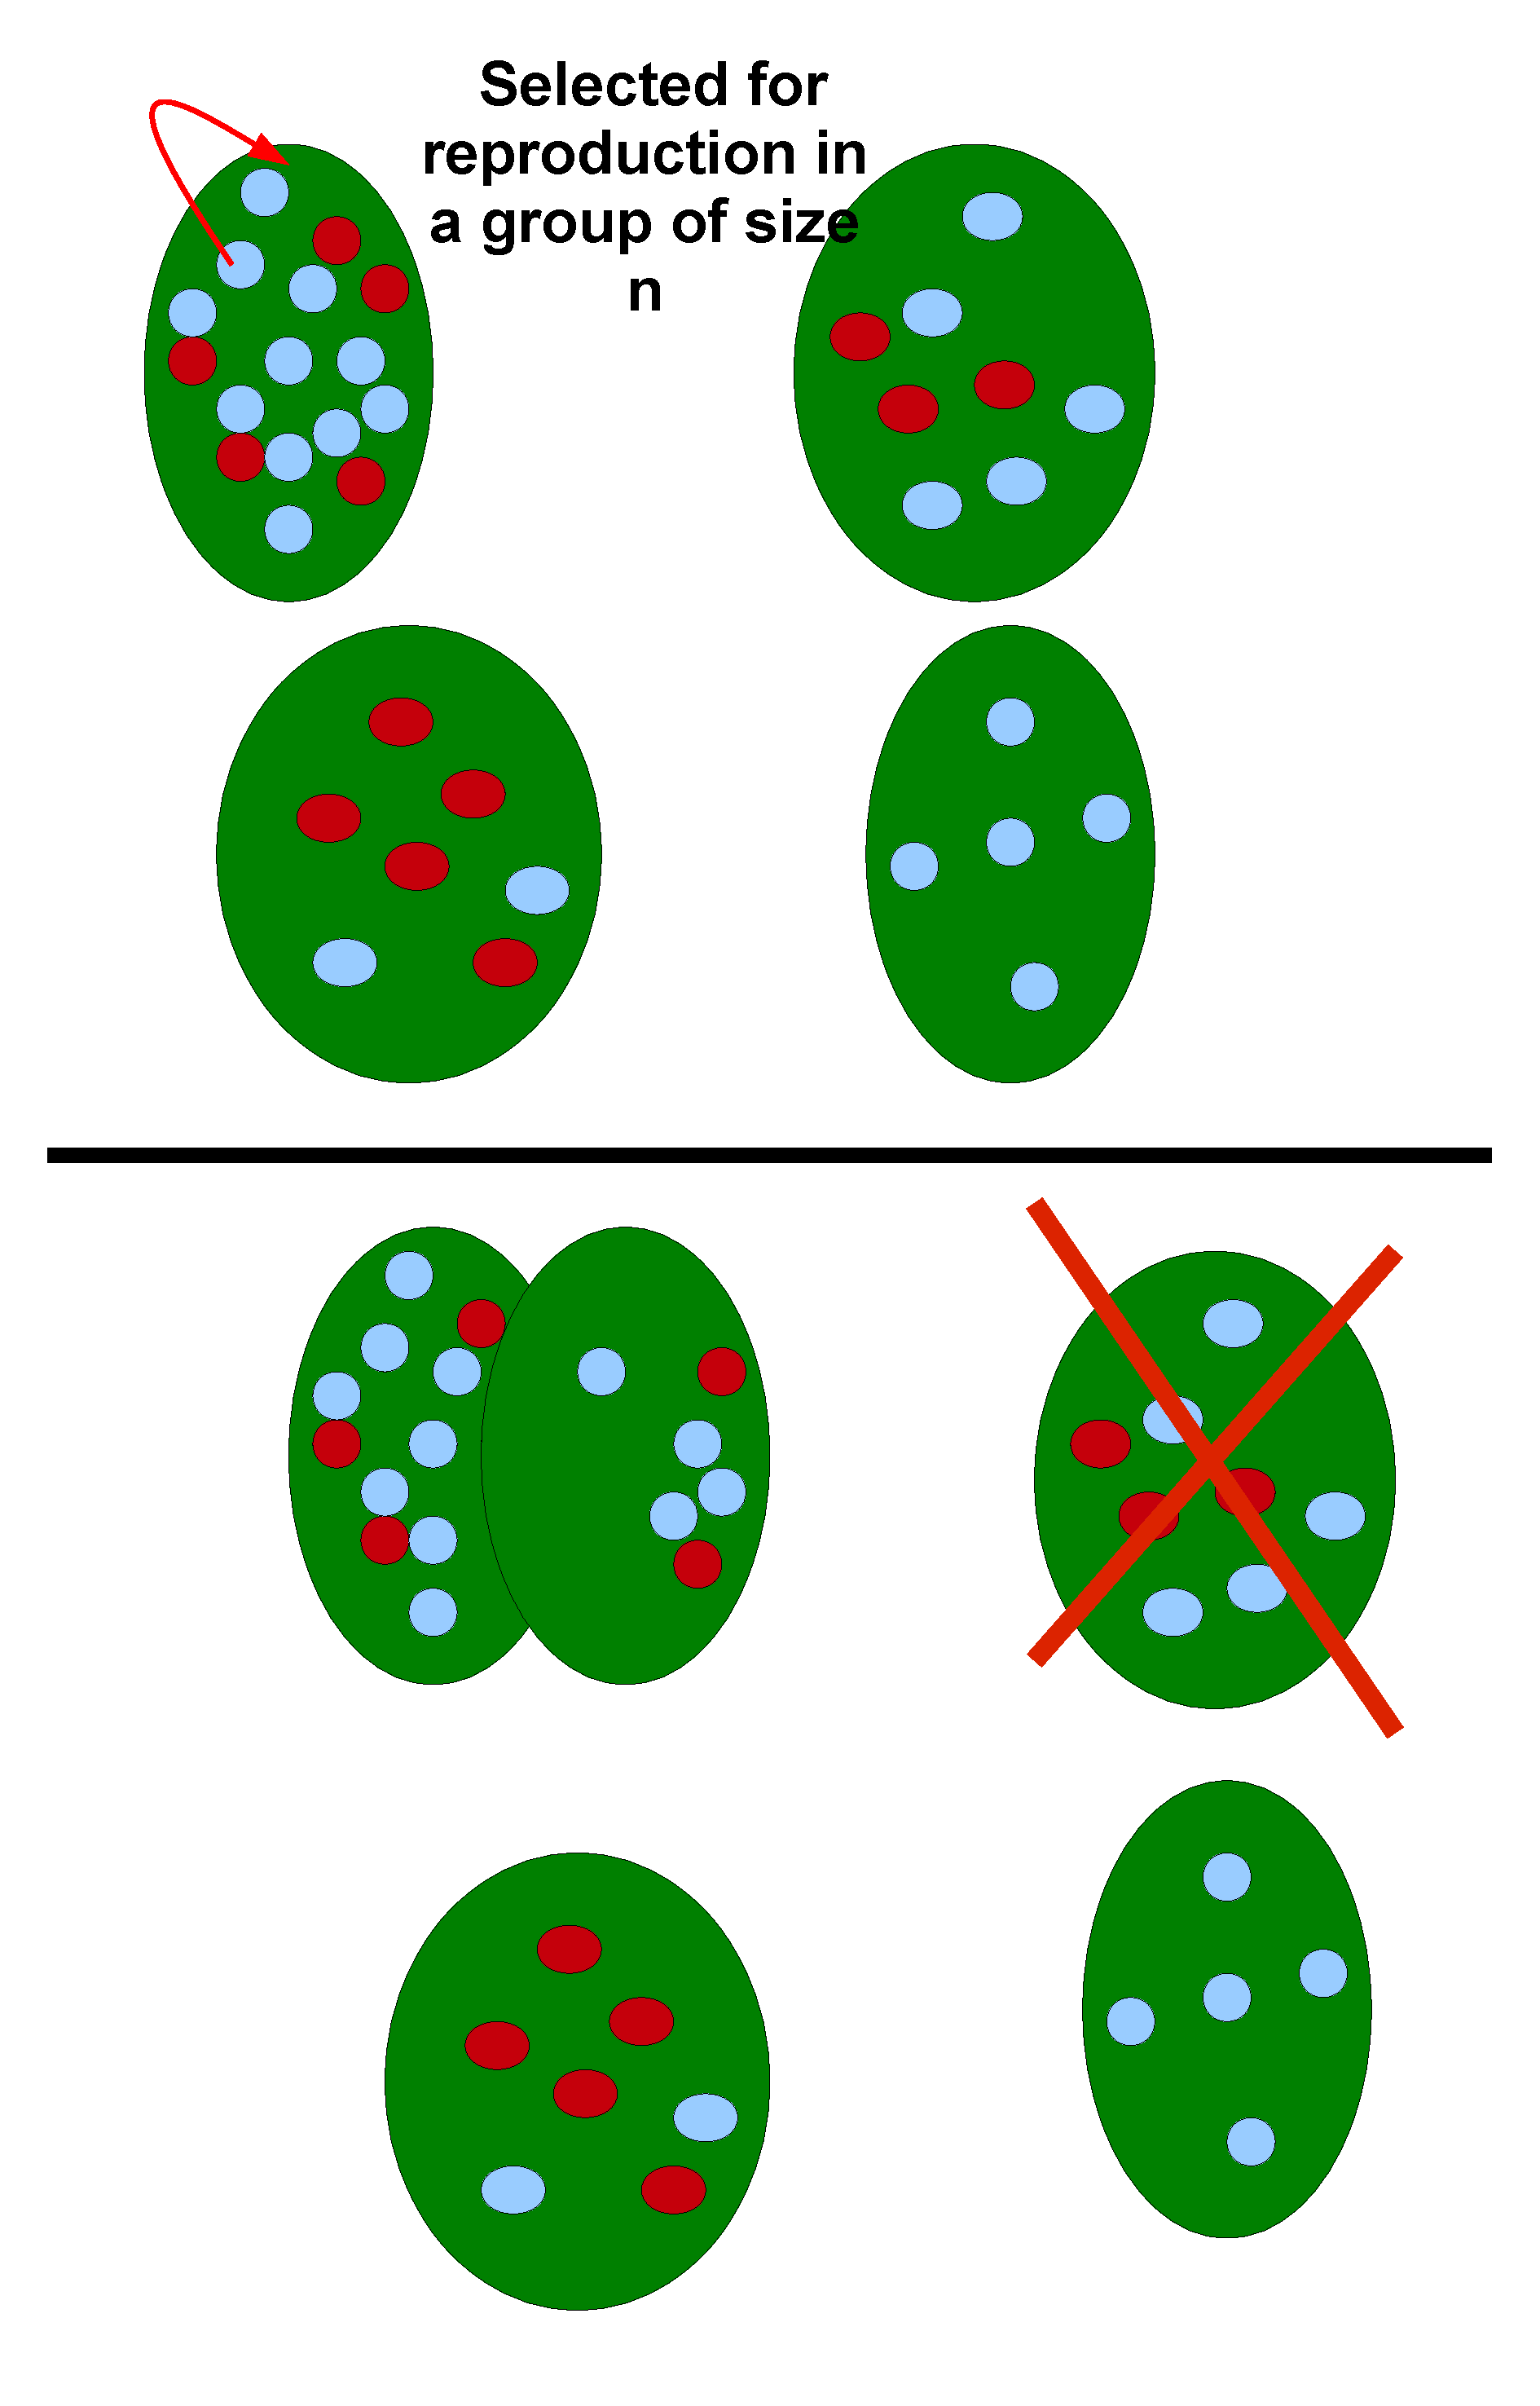
\includegraphics[width=2.5in]{GroupSelection1.pdf} &
b)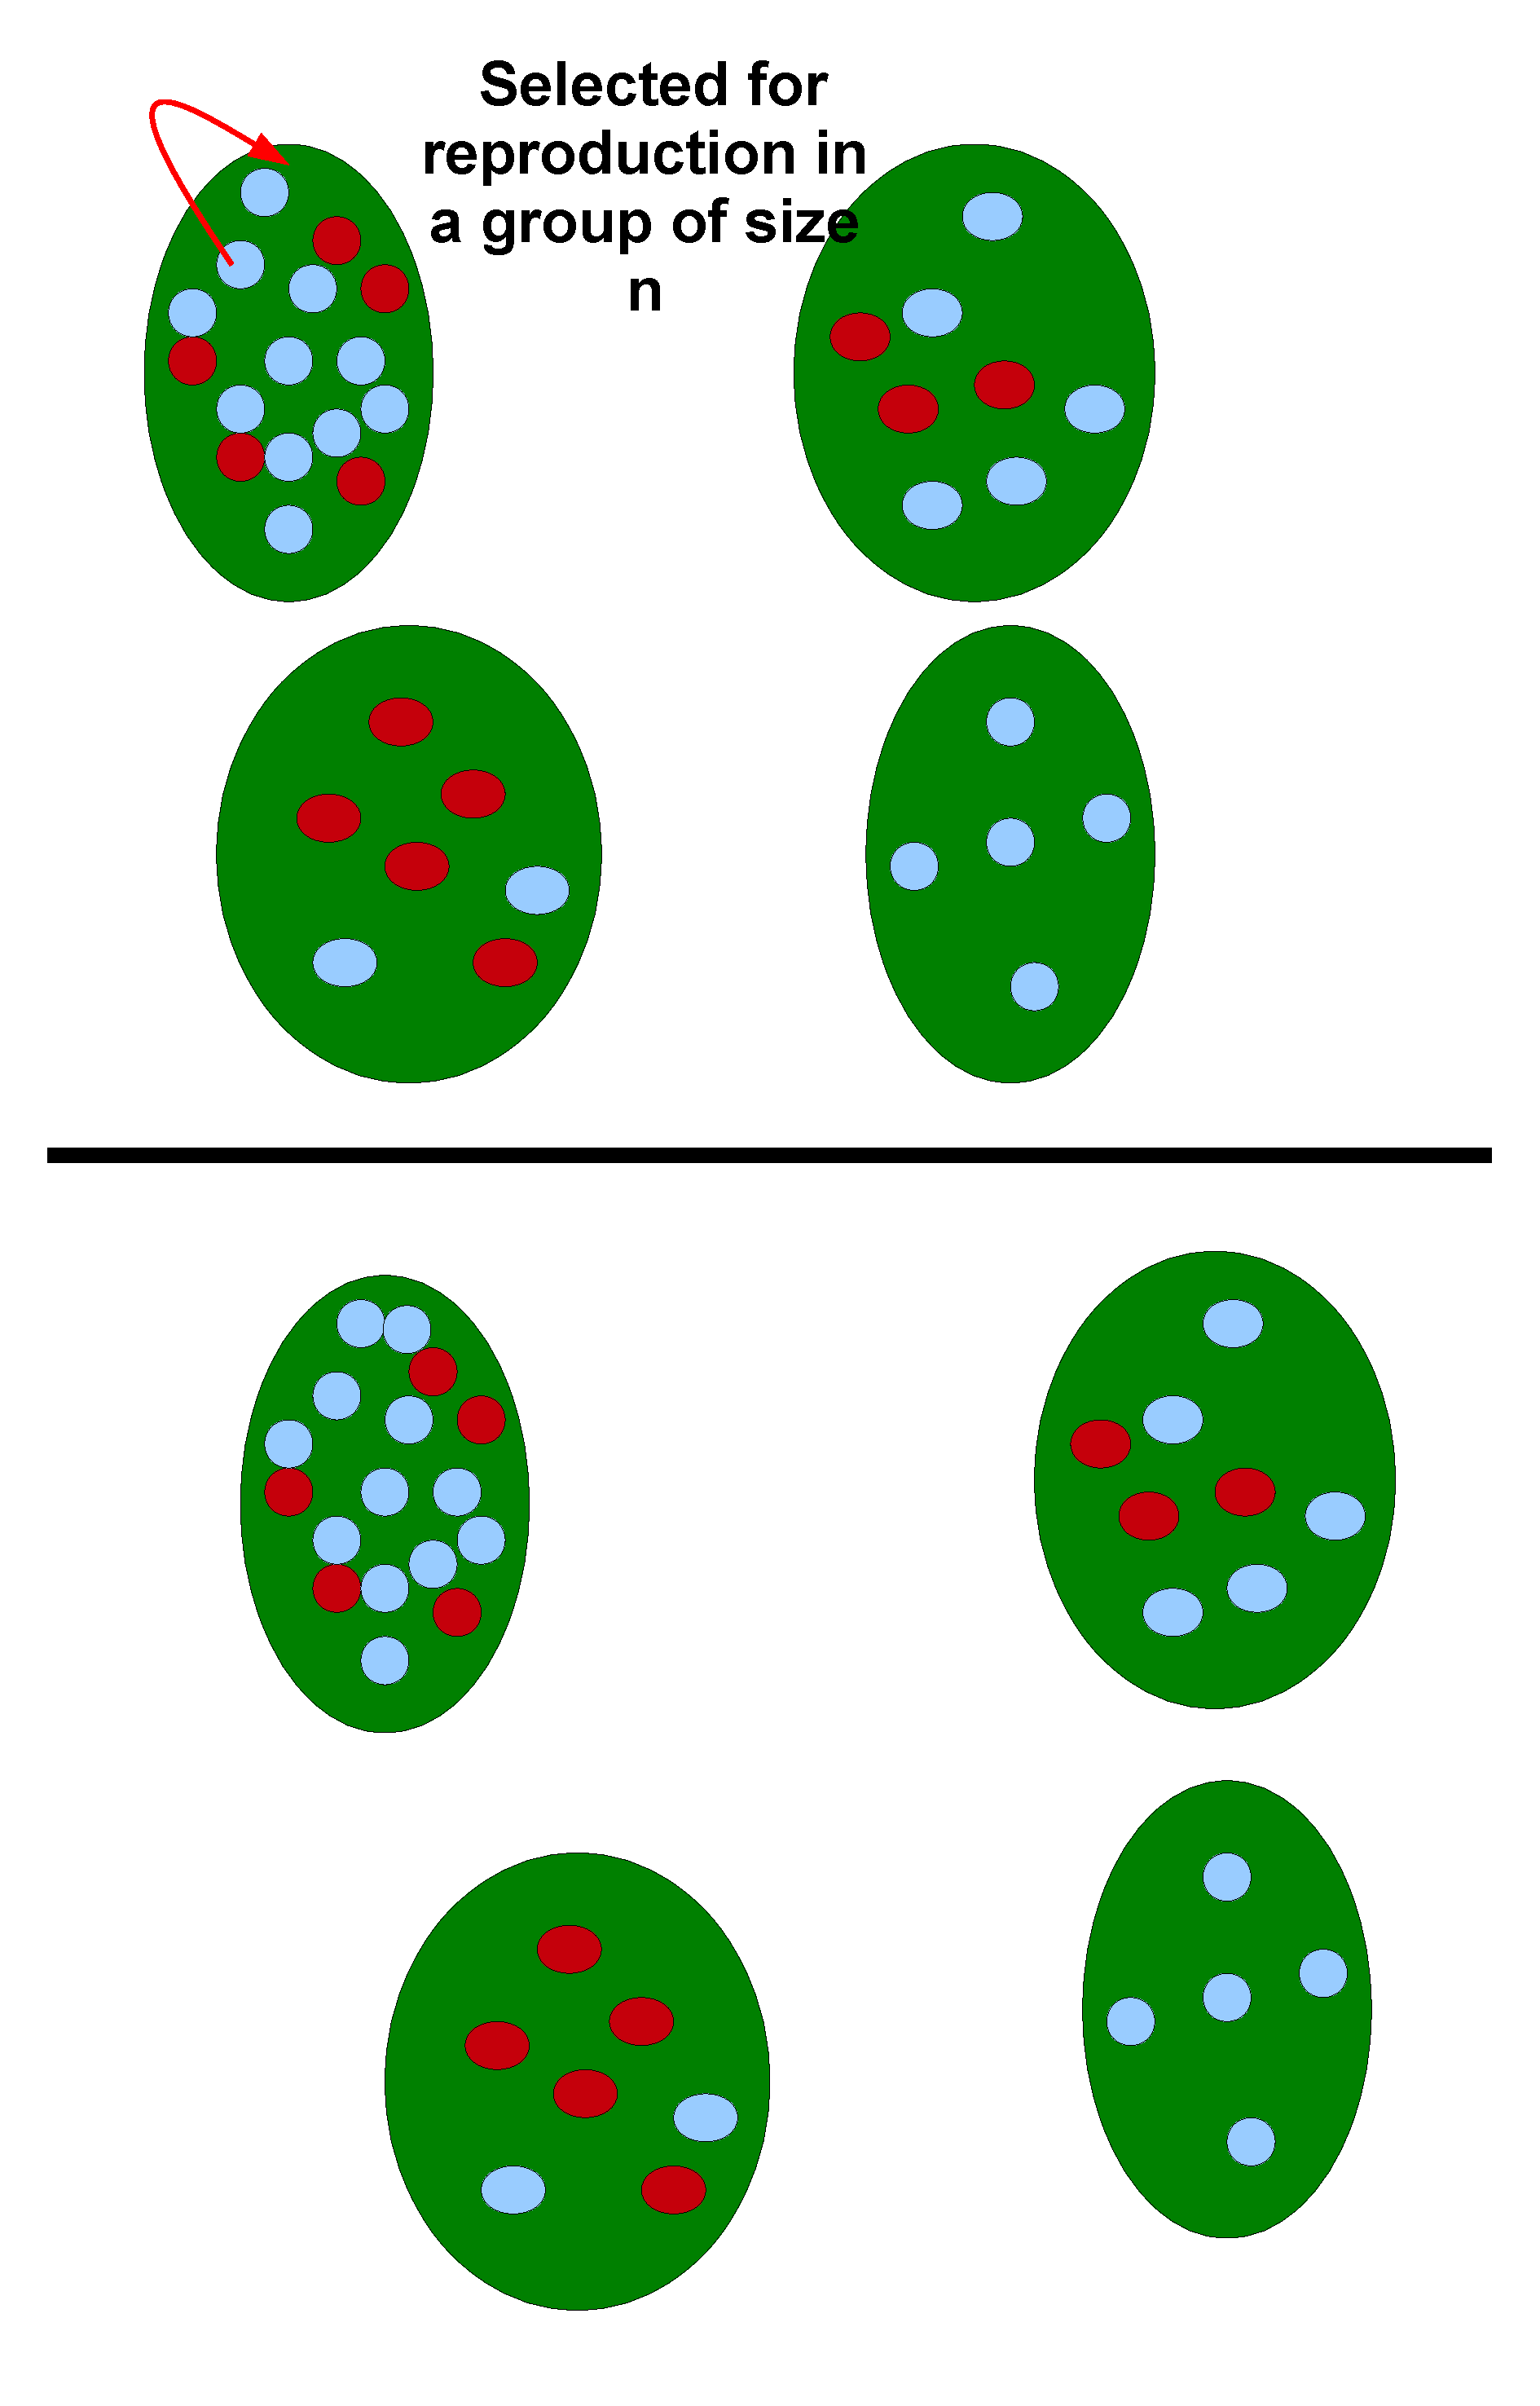
\includegraphics[width=2.5in]{GroupSelection2.pdf}
\end{array}$
\end{center}
\caption{a) . With probability $q$ the group splits in two groups, where generally $q\ll 1$ to allow invasion in groups before any splitting. b) With probability $1-q$ the new offspring take the place of other individual in the group.}
\label{Fig5.2}
\end{figure}

 Fixation probability in group selection is often calculated for an initial single mutant in whole population of $m$ groups of size $n$, with a small $q$\cite{Shoresh2011,Traulsen2006a}. If the splitting probability is small enough, such that the average time for an splitting event is larger than that for fixation of a single mutant in a groups, the fixation probability $\Phi(1)$ in population can be separated in two events: fixation probability $\rho(1,n)$ of a mutant in a group of size $n$, and    fixation probability $\phi(1,m)$ of a single group of mutants in a population of $m$ groups. Thus the risk of dominance of a single mutant is
\begin{equation}
\Phi_1(n,m)=\phi_1(m)\rho_1(n).
\end{equation}
The general form of $\rho_1$ has been already determined in Eq. \eqref{5.14}. A general form for $\phi_1(m)$ can be derived because of the small $q$.
After a mutant of type $A$ has invaded its host group of $n-1$ type $B$ individuals, then the population will be composed  of homogenous groups of $A$ or $B$ individuals. As a result, the transition probability $P_{l,l+1}$ that population changes from $l$ $A$ groups to $l+1$ is the product  of three events:
\begin{itemize}
\item The probability that an individual of type $A$ is selected for reproduction. 
\begin{equation}
\frac{f_A(n)ln}{f_A(n)ln+f_B(0)(l-m)n}.
\end{equation}
\item The probability of splitting $q$
\item The probability that a $B$ group is chosen for elimination.
\begin{equation}
\frac{m-l}{m}
\end{equation}
\end{itemize}
Thus $P_{l,l+1}$ is given by
\begin{equation}
P_{l,l+1}=q\frac{f_A(n)l}{f_A(n)l+f_B(0)(l-m)}\frac{m-l}{m},
\end{equation}
and  $P_{l,l-1}$ by
\begin{equation}
P_{l,l-1}=q\frac{f_B(n)(m-l)}{f_A(n)l+f_B(0)(l-m)}\frac{l}{m},
\end{equation}
In this phase of the process where there are only  homogeneous groups, each group behaves as an individual of fitness $f_{A,B}(n)n$. Consequently the fixation probability of a single mutant of type $A$ in a group has the same form as Eq. \eqref{5.14} for a single mutant in a population of size $m$: 
\begin{equation}\label{5.37}
\phi_{1}(m)=\left(1+ \sum\limits_{k=1}^{m-1}\prod\limits_{l=1}^{k}\frac{f_{B}(0)}{f_{A}(n)}\right)^{-1}
\end{equation} 
Hence, the fixation probability of a single mutant $A$ in a structured population of $m$ groups of maximum size $n$ is given by
\begin{equation}
\Phi_1(n,m)=\left(1+\sum\limits_{k=1}^{n-1}\prod\limits_{j=1}^{k}\frac{f_{B}(j)}{f_{A}(j)}\right)^{-1}\left(1+ \sum\limits_{k=1}^{m-1}\prod\limits_{l=1}^{k}\frac{f_{B}(0)}{f_{A}(n)}\right)^{-1}.
\end{equation} 
In random drift, where a mutant $A$ of fitness $r$ is introduced in a population of $nm-1$ type $B$ individuals with fitness $s$, the respective fixation probability ha an analytical solution, and reduces to   
\begin{equation}
\Phi_1(n,m)=\frac{1-s/r}{1-(s/r)^{n}}\frac{1-s/r}{1-(s/r)^{m}}.
\end{equation}
This is can be corroborated with the stochastic simulation data in (Figure \ref{Fig5.3}).

From this expression  some important features of a structured population can be seen\cite{Traulsen2005}. Comparing the fixation probability $\rho_{1}(r,nm)$ of a single mutant $A$ in a unstructured population of size $nm$ with that for group selection, $\Phi_{1}(r,n,m)$, we see that  for $s<r$ we have $\Phi_{r,n,m}\leqslant \rho_1(r,nm)$, which means that an advantageous mutant is  less likely to be fixated in a structured population. In contrast, for $r<s$ we have $\Phi_{r,n,m}\geqslant \rho_1(r,nm)$, which means that a disadvantageous mutant is more likely to fixate in a structured population. This  shows that the process of group splitting works as a suppressor of individual selection.
 
\begin{figure}[H]\label{Fig5.3}
        \begin{center}
  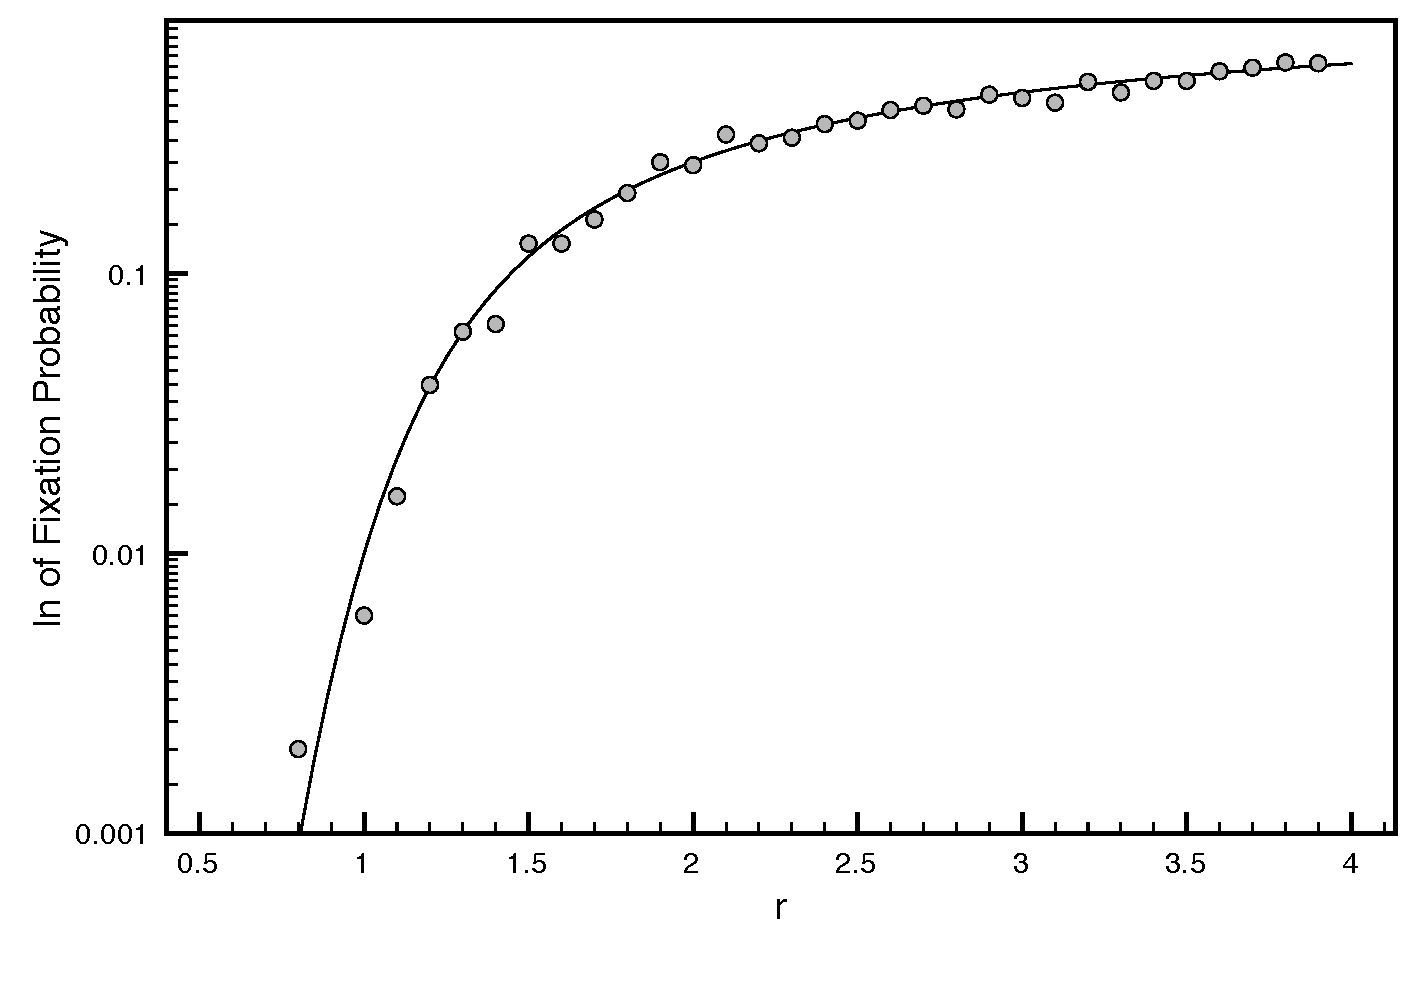
\includegraphics[width=11cm,height=8cm]{m10n10q0001.pdf}
     \end{center}
      \caption{Group selection for no interaction games. $n=10$, $m=10$ and $q=0.001$} 
   \end{figure}
 Now we will study the case of interaction games, where there are social interactions among the individuals of each group. In this system we have type $C$(cooperators) individuals and type $D$(defectors), with the payoff matrix.
 \begin{equation}
 \bordermatrix{~ & C & D \cr
             C & R & S \cr
              D & T & P \cr} 
 \end{equation} 
 and expected fitness by individual
  \begin{equation}
  f_{C}(i)=1-w+w\pi_{C}(i) \;\;\;  f_{D}(i)=1-w+w\pi_{D}(i)
  \end{equation}
 The fixation probability for a single cooperator in a group of $n-1$ defectors, for weak selection, has been already determined in Eq. \eqref{5.29}. Thus
 \begin{equation}
 \rho_{D}(n)=\frac{1}{n} -\frac{w}{6n}\left[ (T-R+2P-2S)n-(T+2R-4P+S)\right].
 \end{equation}
Fixation probability $\phi_{C}(m)$ of a single group of cooperators can be compute using Eq. \eqref{5.37}, which for weak selection is\cite{Traulsen2006a}
\begin{equation}
\phi_{D}(m)=\frac{1}{m}\left[1+\frac{w}{2}(m-1)(R-P)\right].
\end{equation} 
Therefore the fixation probability of a single mutant in a structure population of $m$ groups of size $n$ is given by
\begin{equation}
\Phi_{C}(n,m)=\frac{1}{mn}\left[1+w\left(-\frac{(T-R+2P-2S)n-(T-4R+2P+S)}{6}+\frac{m-1}{2}(R-P)\right)\right].
\end{equation}
Using Eq. \eqref{5.31} for a single defector in a group, and the fixation probability of a single defector group,
\begin{equation}
\phi_{D}(m)=\frac{1}{m}\left[1-\frac{w}{2}(m-1)(R-P)\right],
\end{equation}
the fixation probability of a single defector in structured population is
\begin{equation}
\Phi_{D}()n,m)=\frac{1}{nm}\left[1+w\left(\frac{1}{6}((2T-2R+P-S)n-(T-4R+2P+S)) +\frac{m-1}{2}(R-P)\right)\right].
\end{equation}
Now let us compare these analytical approximations with the pair interaction stochastic simulation. For this propose  a prisoner's dilemma  game will be used,  with the payoff matrix
\begin{equation}
\bordermatrix{~ & C & D \cr
             C & b-c & -c \cr
              D & b & 0 \cr},
\end{equation}
where $c$ represents the cost of cooperating and $b$ the benefit that an individual gets from the cooperation of its partner. In (Figure \ref{Fig5.4})  the population fraction as a function of time steps for group selection is shown, where the peaks represents the splitting of a group, the division of a group of size $n$ replaces another group of size $n$ most likely by a new group of $n/2$ individuals, which explains the abrupt changes in population.     
\begin{figure}[H]\label{Fig5.4}
        \begin{center}
  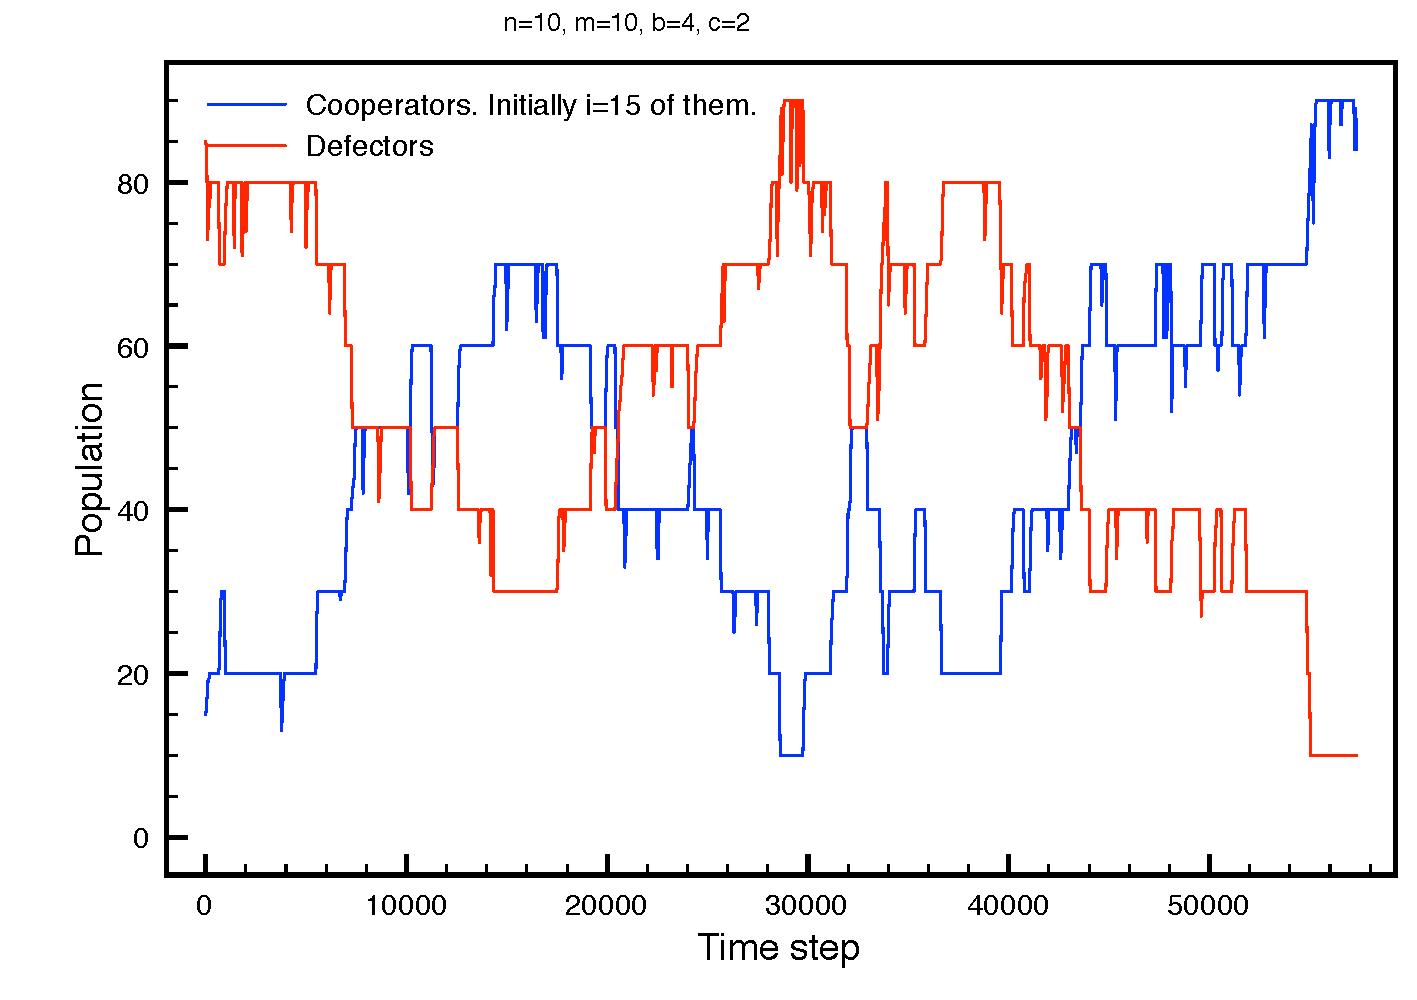
\includegraphics[width=11cm,height=8cm]{groupselection.pdf}
     \end{center}
      \caption{The peaks are the splitting of a group. $q=0.001$} 
   \end{figure}
Now let us analyze the conditions where a cooperator is more likely to invade a structure population of defectors than a single defector invade  a population of cooperators. In other words, what are the values of the ratio $c/b$ where $\Phi_{C}(n,m)\geq \Phi_{D}(n,m)$. For $b$ and $c$, the fixation probabilities simplify to
\begin{equation}
\Phi_{C}(n,m)=\frac{1}{mn}\left[1+w\left(-\frac{1}{6}(3cn+3(c-b))+\frac{m-1}{2}(b-c)\right)\right] 
\end{equation}
\begin{equation}
\Phi_{D}(n,m)=\frac{1}{mn}\left[1+w\left(\frac{1}{6}(3cn+3(c-b))-\frac{m-1}{2}(b-c)\right)\right].
\end{equation}
The inequality reduces to
\begin{equation}
(m-1)(b-c)\geq cn + c-b ,
\end{equation}
which can be written as
\begin{equation}
\frac{b}{c}\geq \frac{n}{m-2} + 1.
\end{equation}
From this inequality it is inferred  that the benefit to cost ratio where a cooperator is most likely to invade than a defector, depends on the structure of population. This inequality is compared in the next figure with data obtained from a group selection simulation for different values of $m$ (Figure \ref{}).
\begin{figure}[H]\label{}
        \begin{center}
  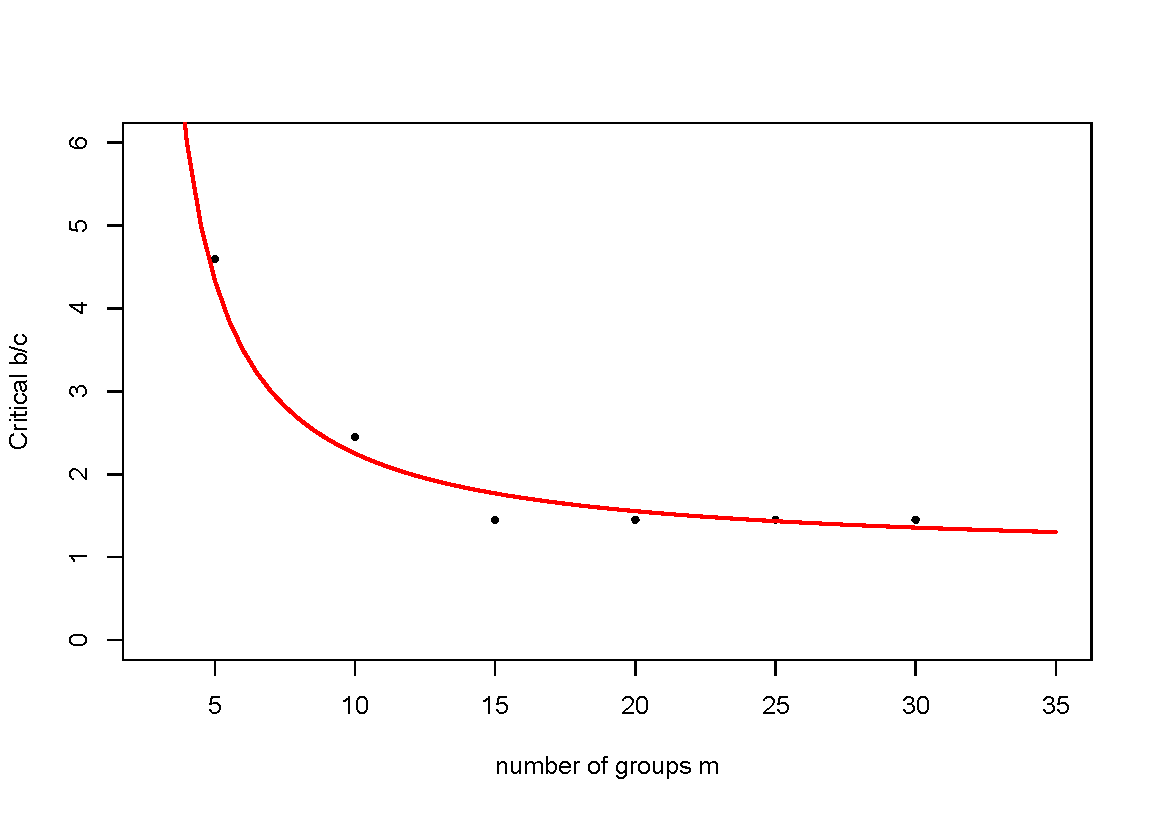
\includegraphics[width=11cm,height=8cm]{bcratio.pdf}
     \end{center}
      \caption{Group selection curve for invasion, $q=0.001$, $w=0.1$ and $n=10$.} 
   \end{figure}
%%% Local Variables: 
%%% mode: latex
%%% TeX-master: "../thesis"
%%% End: 
